%\documentclass{article}
%\usepackage{fixltx2e}
%\usepackage{graphicx}
%\usepackage{caption}
%\usepackage{subcaption}

%\begin{document}

\documentclass{article}
\usepackage{graphicx}
\usepackage{caption}
\usepackage{subcaption}

\begin{document}
\listoffigures 
\newpage
\begin{frame}


\begin{figure}[!tbp]
  \centering
	\fbox{  
	 	\begin{subfigure}[b]{0.27\textwidth}
	 	\centering
	    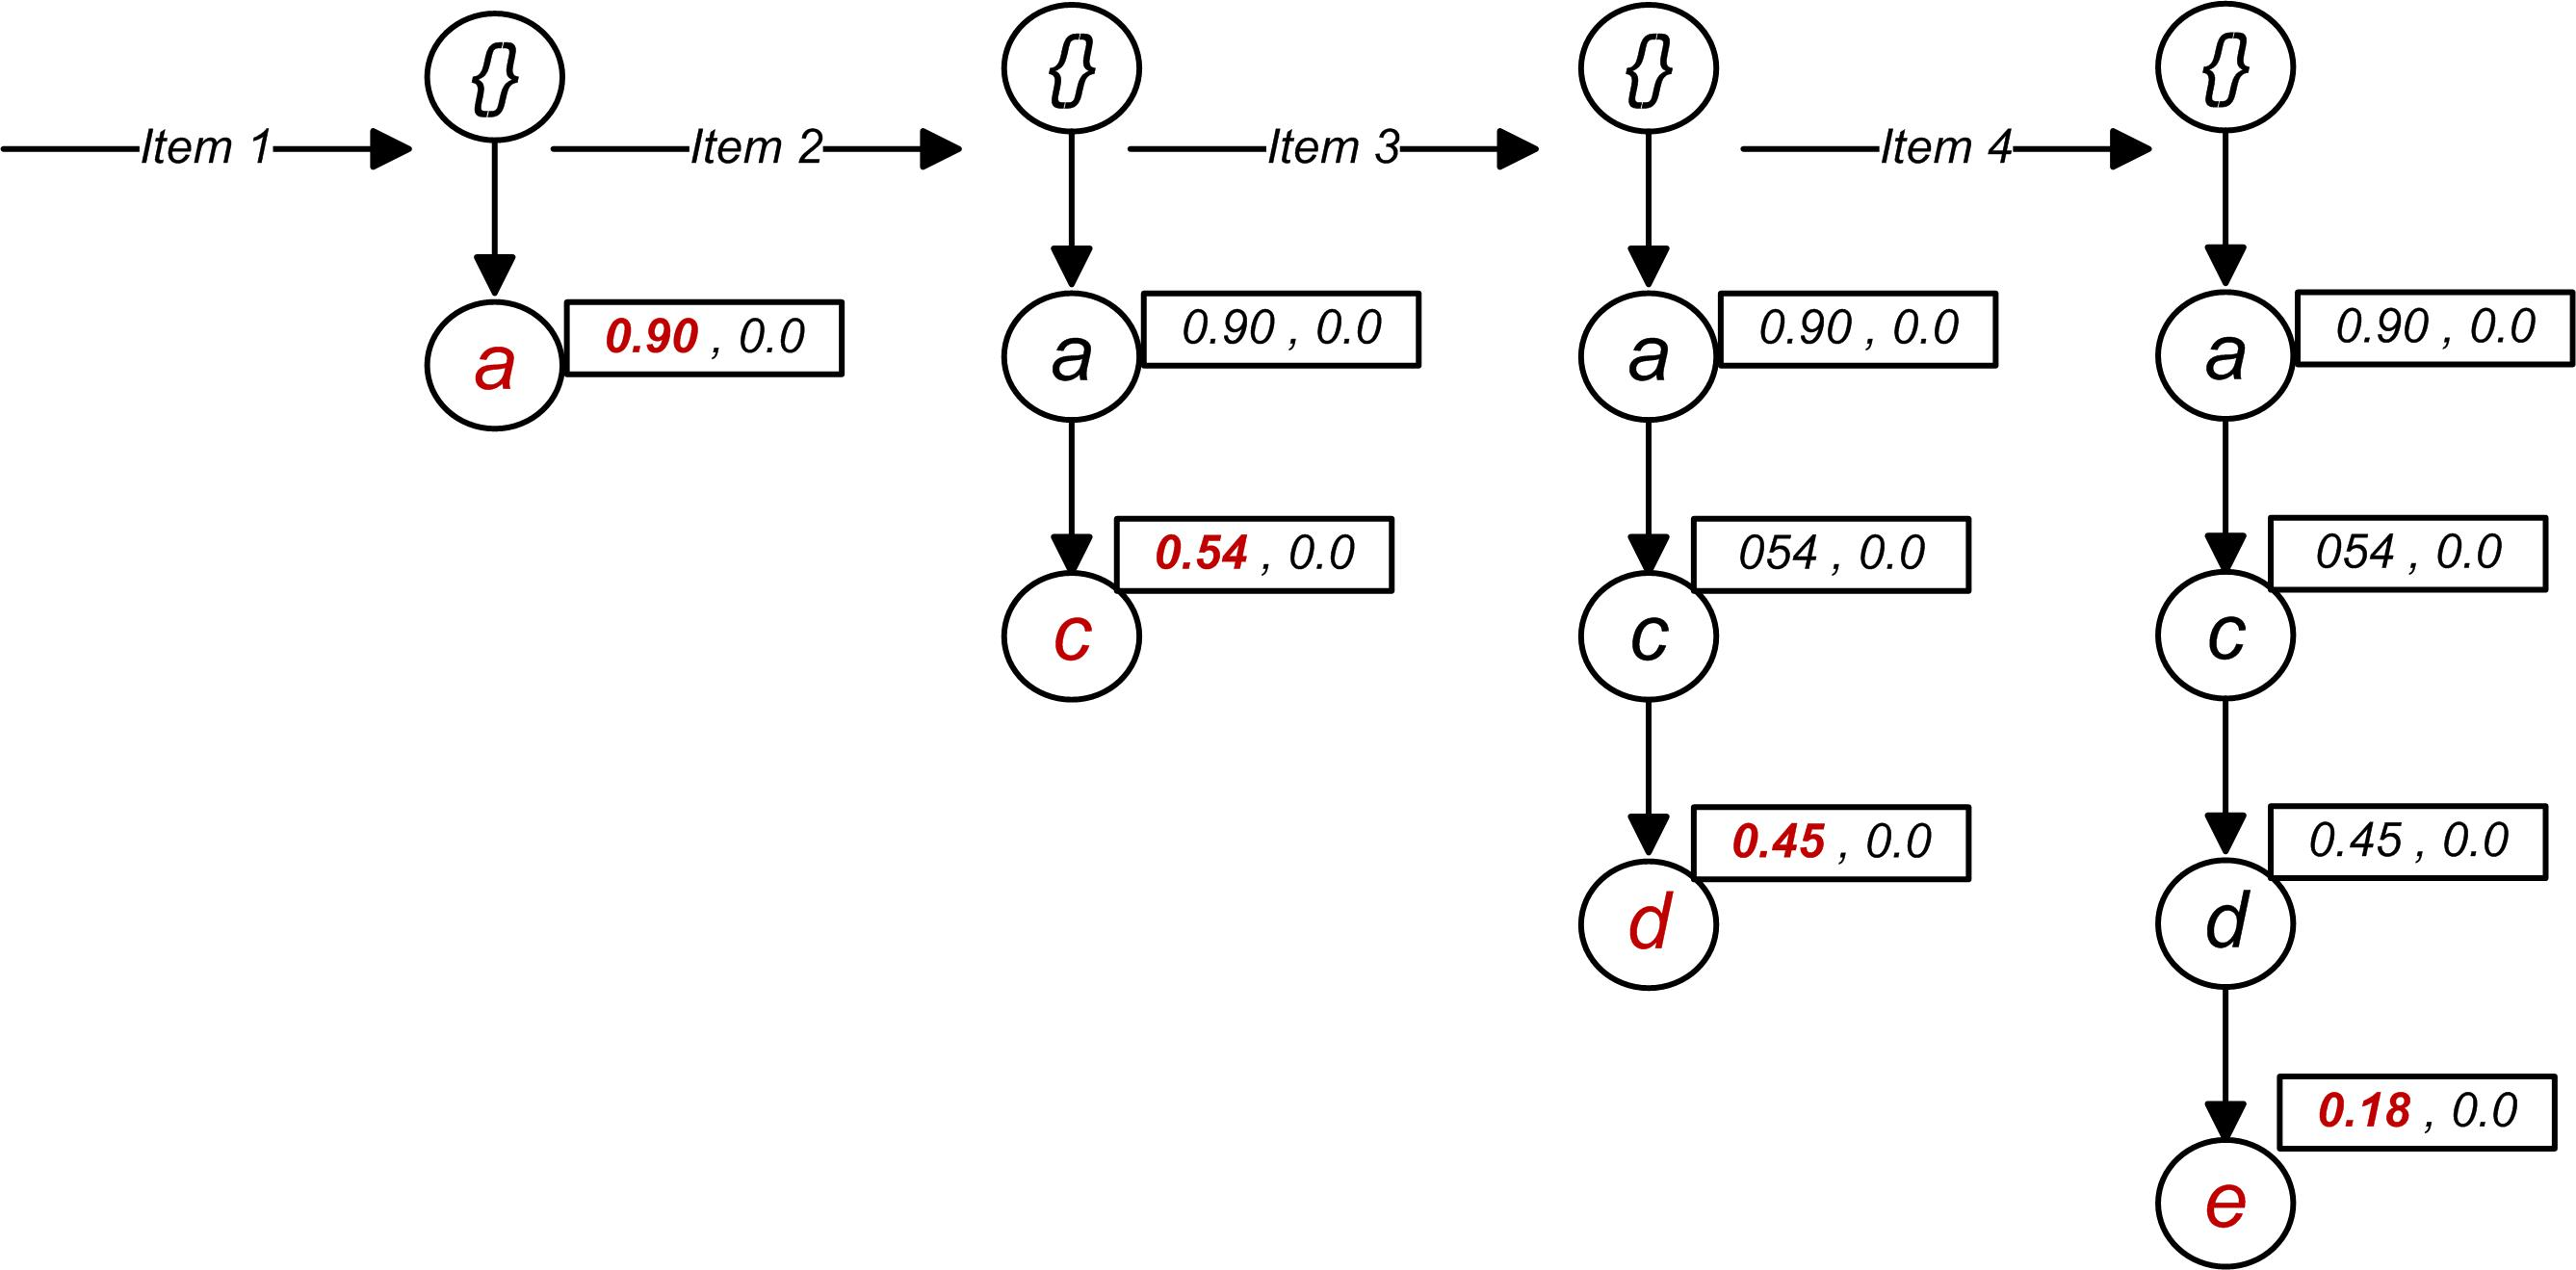
\includegraphics[width=\textwidth,height=3cm]{../images/sim_01.jpg}
	    \caption{T1}
		\end{subfigure}
	}
  \hfill
  	\fbox{  
	 	\begin{subfigure}[b]{0.27\textwidth}
	 	\centering
	    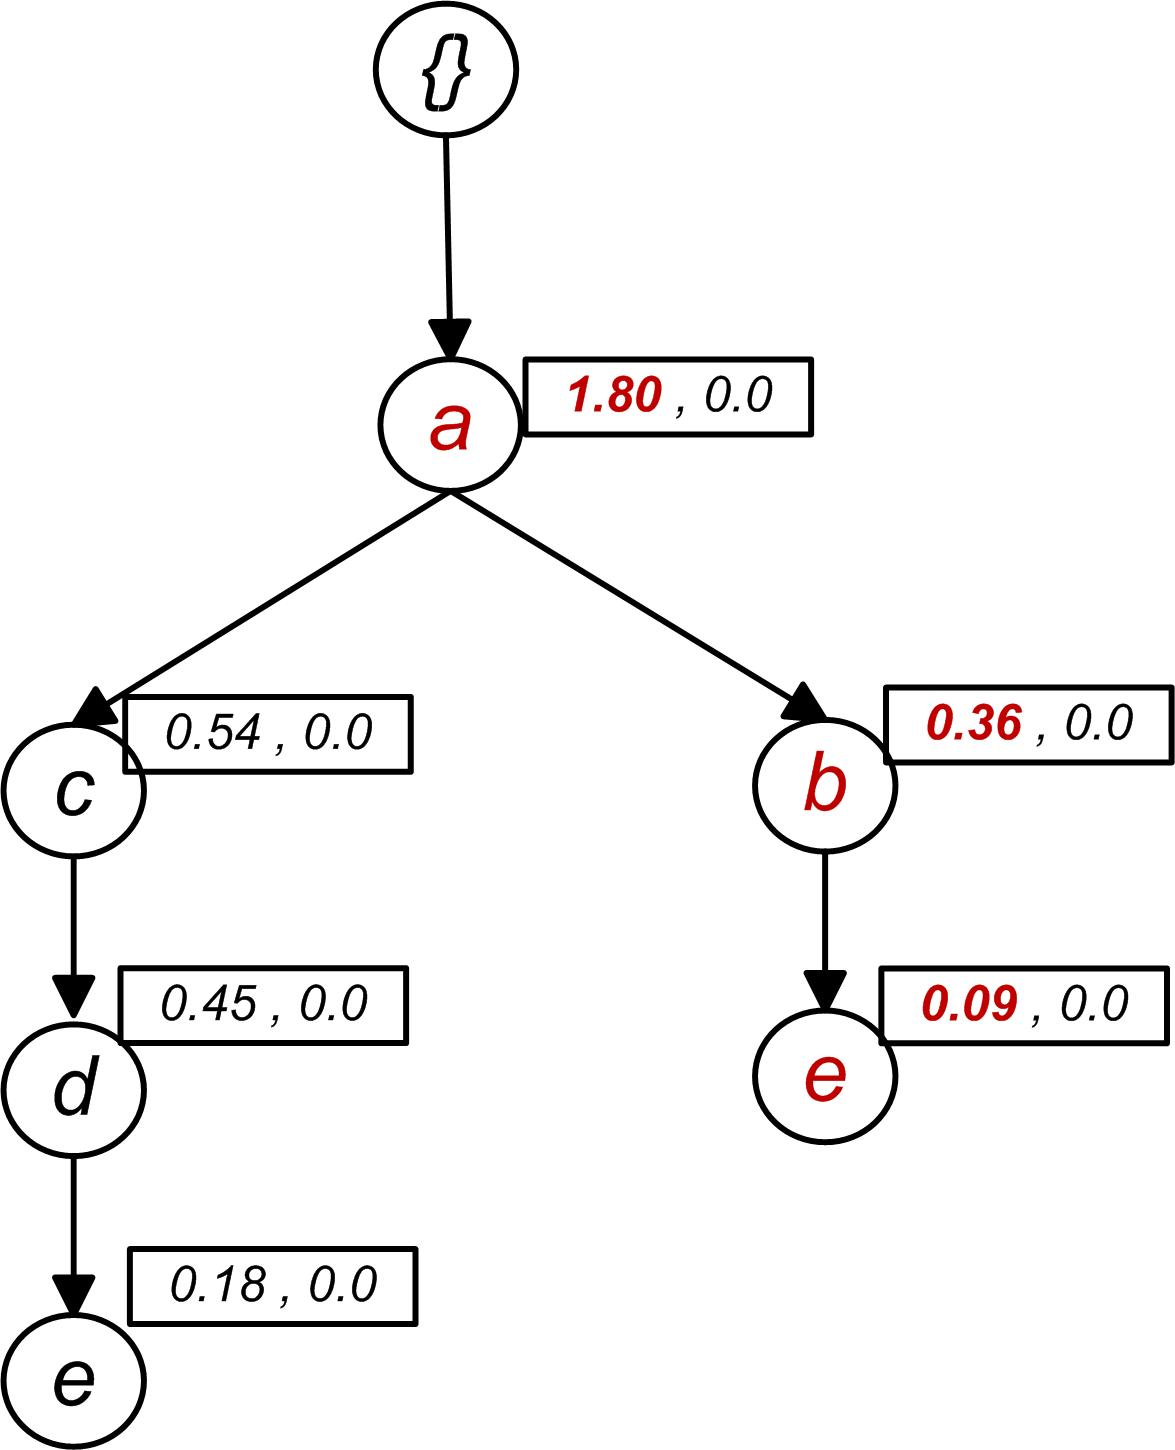
\includegraphics[width=\textwidth,height=3cm]{../images/sim_02.jpg}
	    \caption{T2}
		\end{subfigure}
	}
	\hfill
  \fbox{  
	 	\begin{subfigure}[b]{0.27\textwidth}
	 	\centering
	    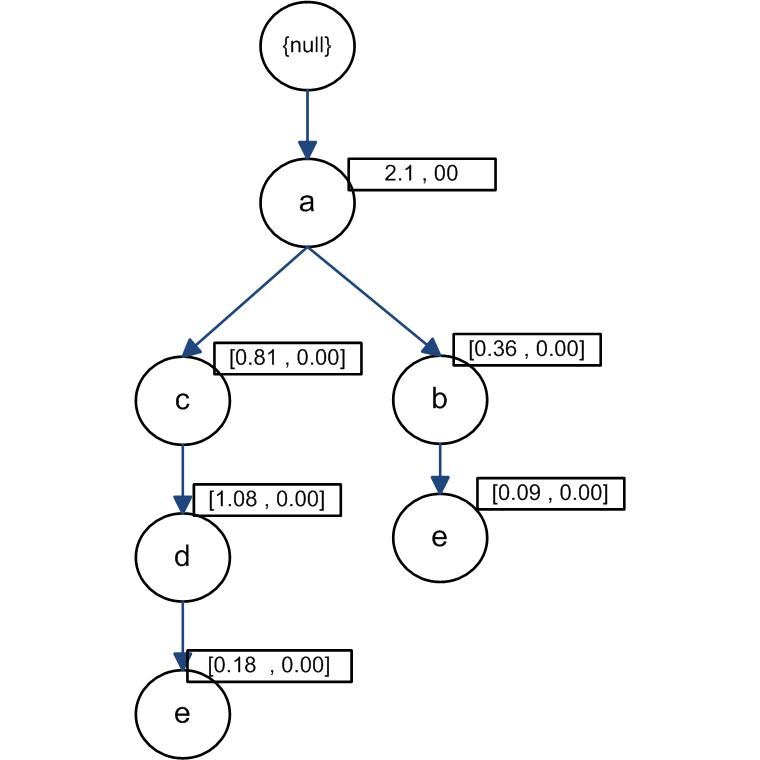
\includegraphics[width=\textwidth,height=3cm]{../images/sim_03.jpg}
	    \caption{T3}
		\end{subfigure}
	}
 \caption{Window 1}
\end{figure}
\end{frame}

\begin{frame}

\begin{figure}[!tbp]
  \centering
	\fbox{  
	 	\begin{subfigure}[b]{0.27\textwidth}
	 	\centering
	    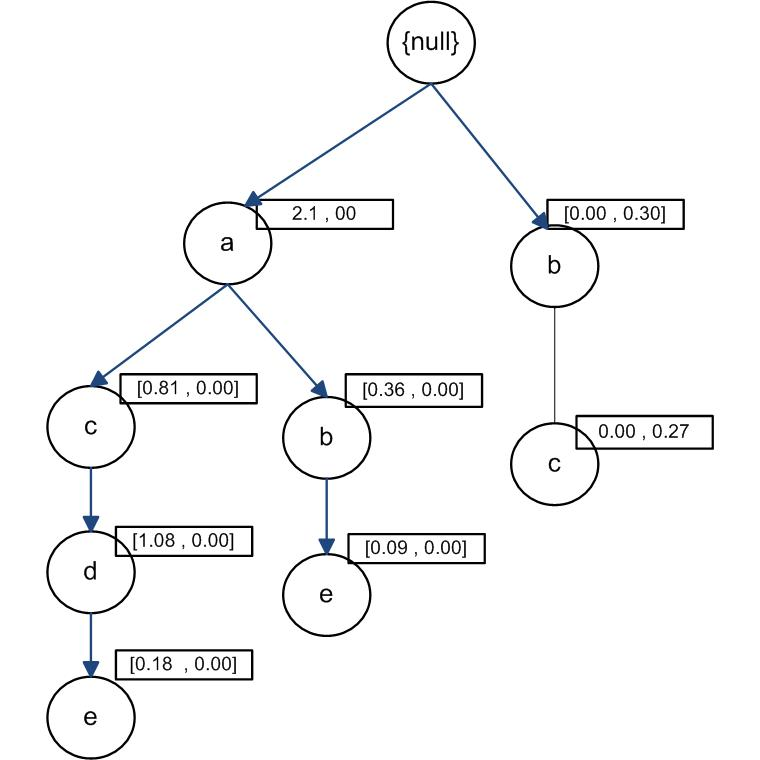
\includegraphics[width=\textwidth,height=3cm]{../images/sim_04.jpg}
	    \caption{T4}
		\end{subfigure}
	}
  \hfill
  	\fbox{  
	 	\begin{subfigure}[b]{0.27\textwidth}
	 	\centering
	    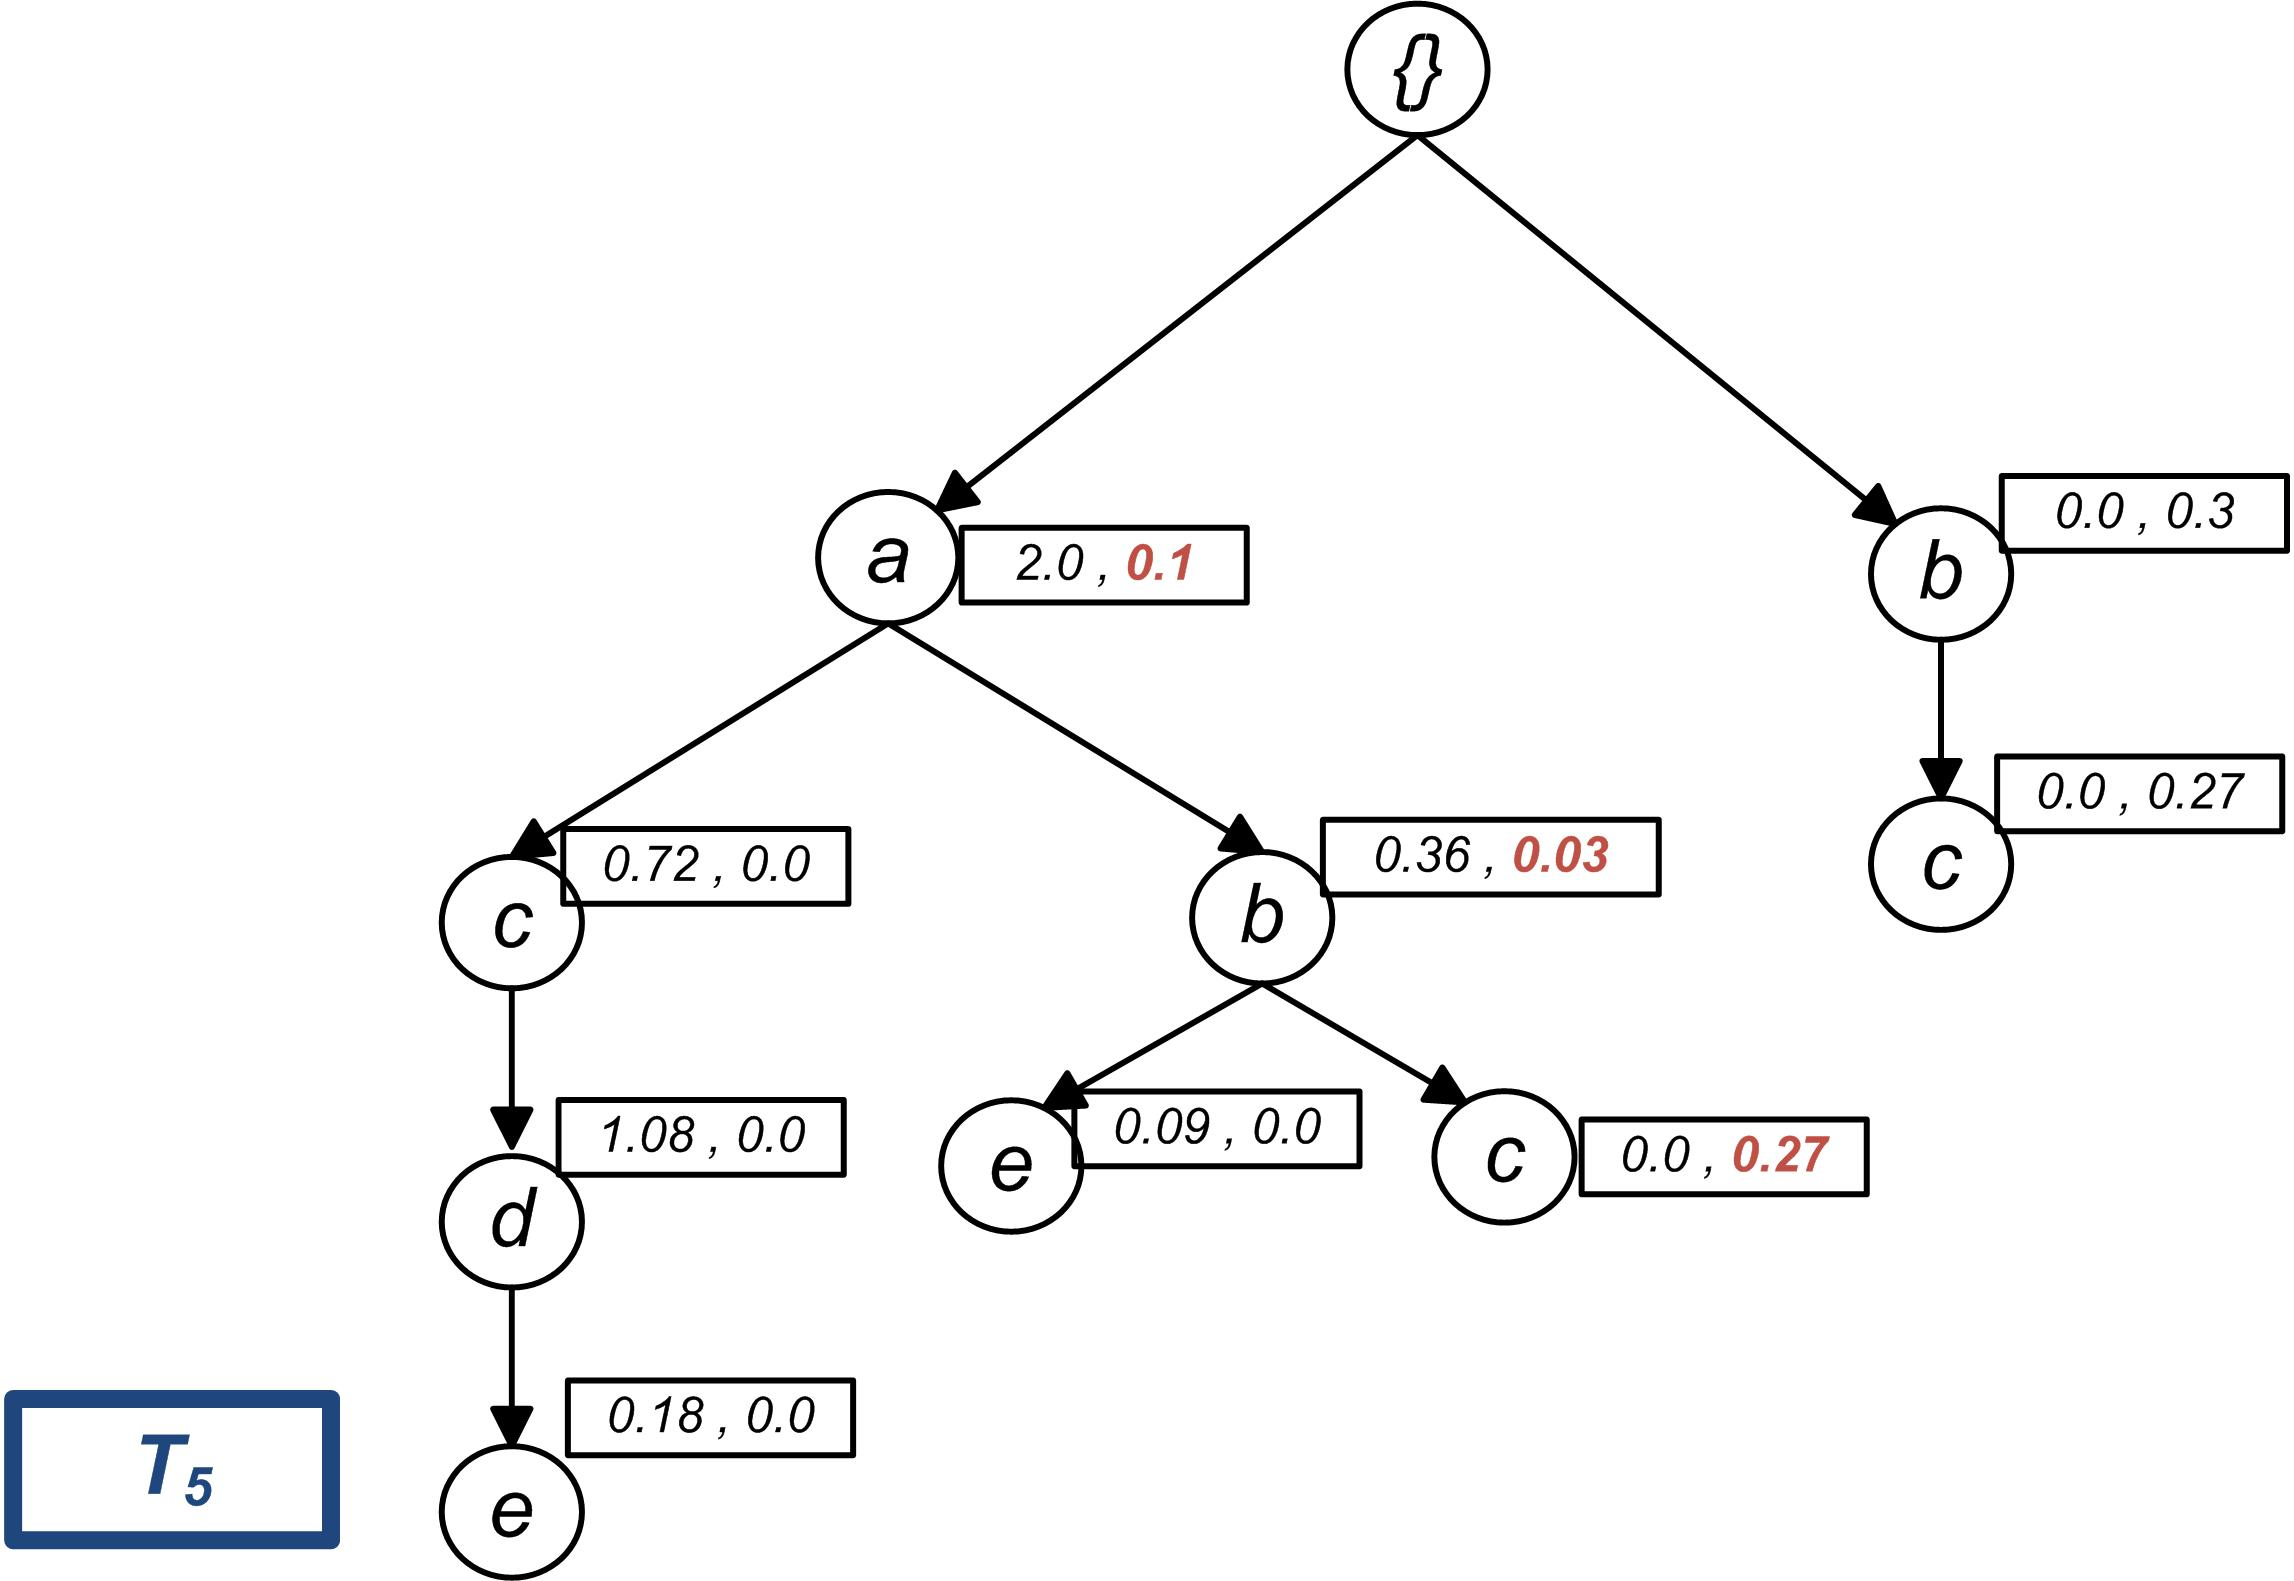
\includegraphics[width=\textwidth,height=3cm]{../images/sim_05.jpg}
	    \caption{T5}
		\end{subfigure}
	}
	\hfill
  \fbox{  
	 	\begin{subfigure}[b]{0.27\textwidth}
	 	\centering
	    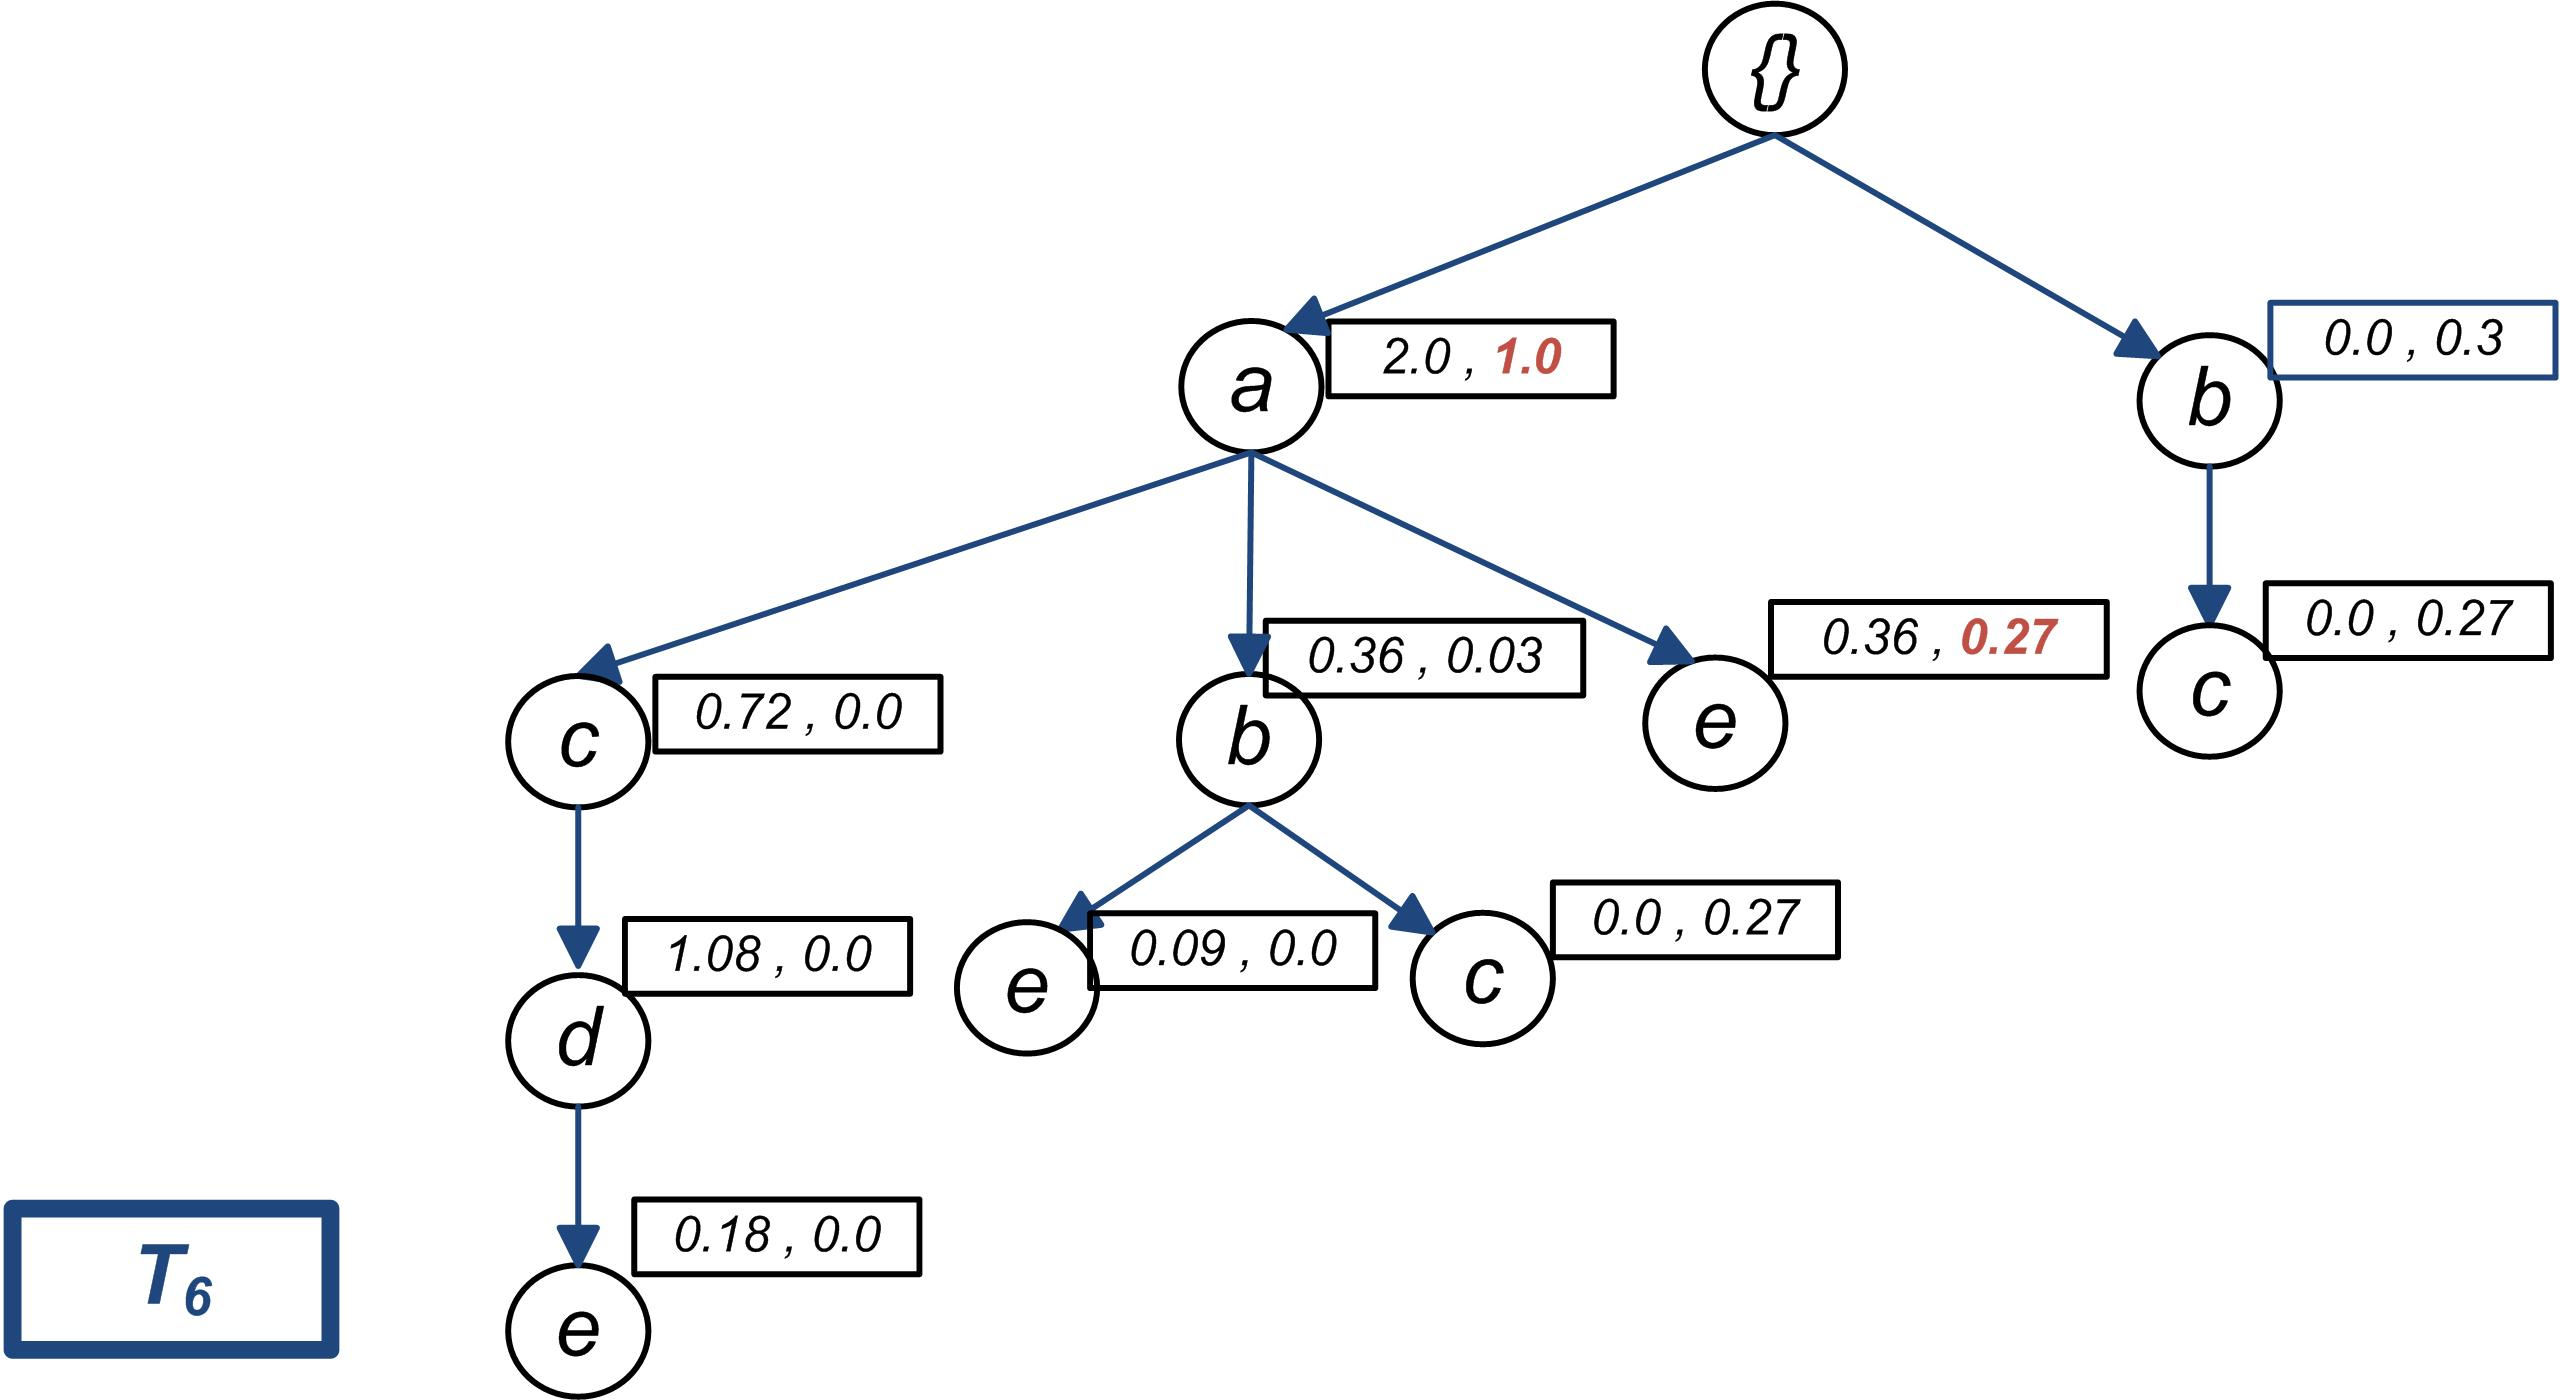
\includegraphics[width=\textwidth,height=3cm]{../images/sim_06.jpg}
	    \caption{T6}
		\end{subfigure}
	}
 \caption{Window 2}
\end{figure}
\end{frame}

\begin{frame}

\begin{figure}[!tbp]
  \centering
	\fbox{  
	 	\begin{subfigure}[b]{0.45\textwidth}
	 	\centering
	    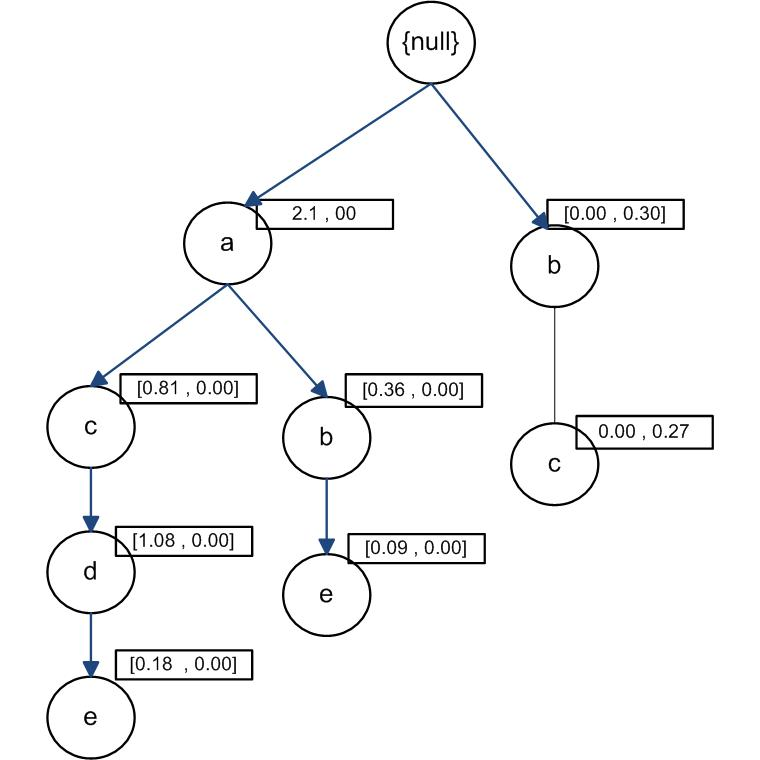
\includegraphics[width=\textwidth,height=5.5cm]{../images/sim_04.jpg}
	    \caption{Completed Window}
		\end{subfigure}
	}
  \hfill
  	\fbox{  
	 	\begin{subfigure}[b]{0.45\textwidth}
	 	\centering
	    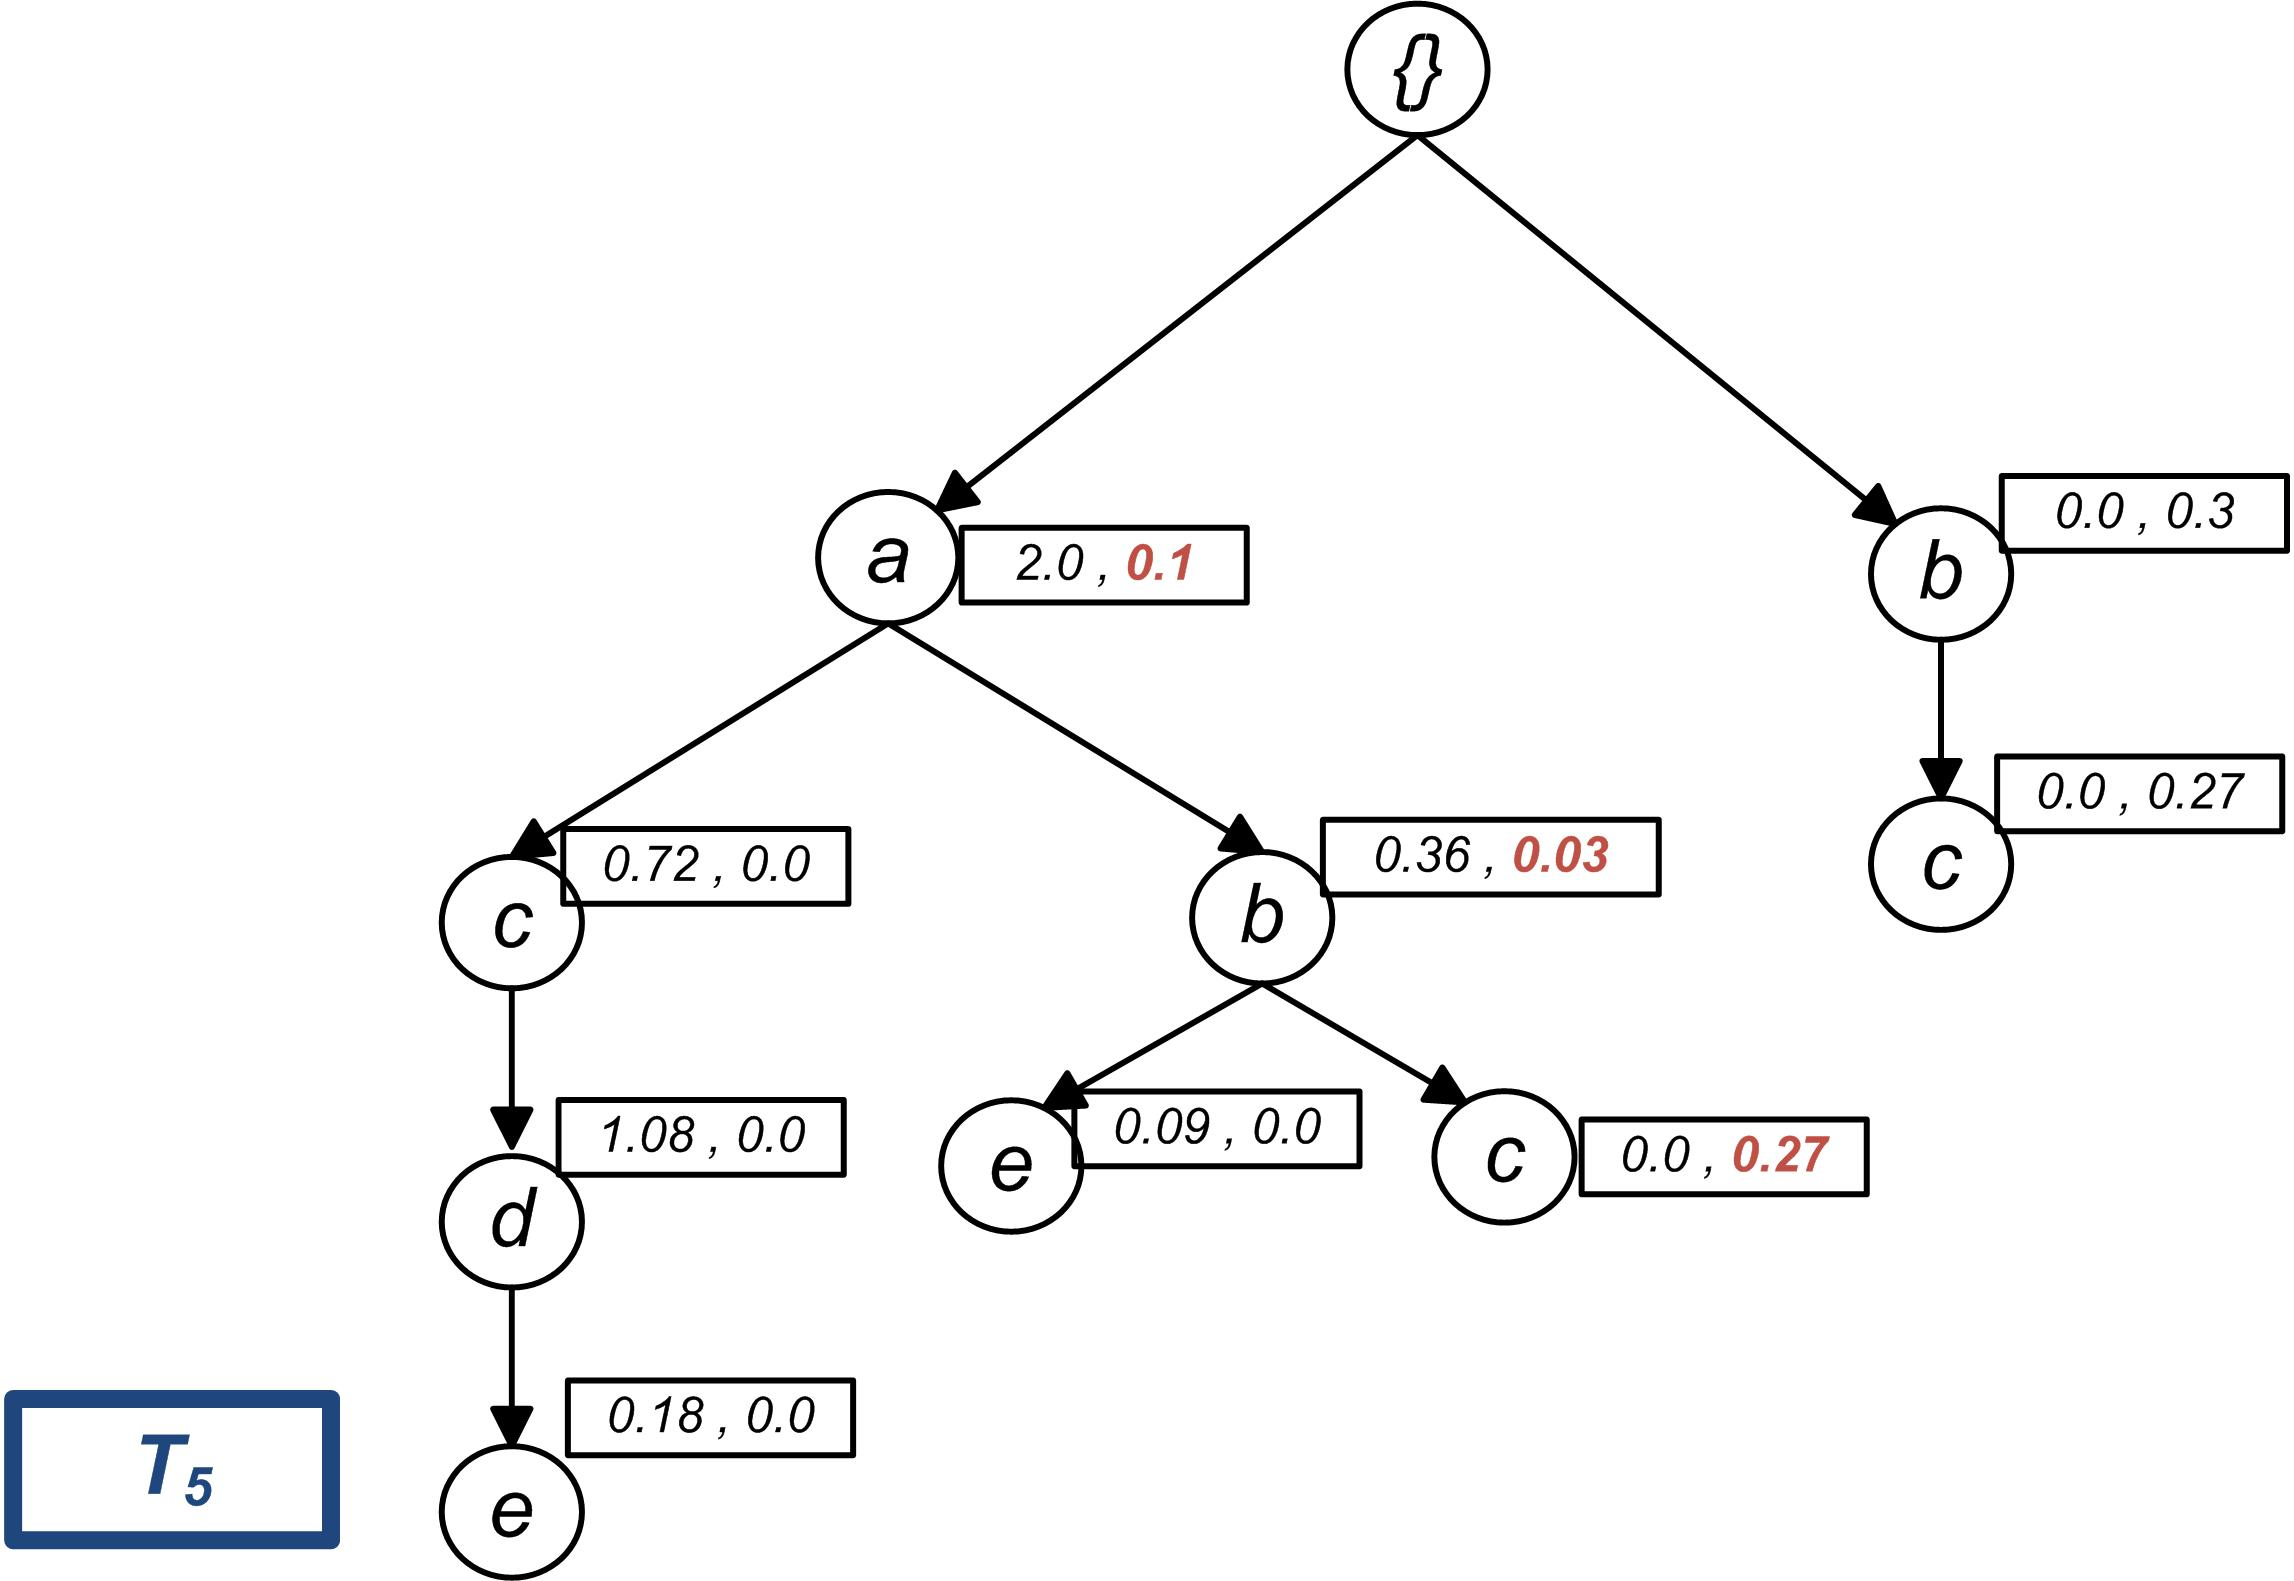
\includegraphics[width=\textwidth,height=5.5cm]{../images/sim_05.jpg}
	    \caption{Window after Slide}
		\end{subfigure}
	}
	\hfill
  
 \caption{After Sliding Window 2}
\end{figure}
\end{frame}

\end{document}
\paragraph*{}
In this section we will describe about our tree construction \emph{US-tree}. We have describe earlier about our batch and window. A batch should be inserted into the tree in it's own window slot. After inserting all batches of to full the window, the window shall be complete and be ready to mine. We said earlier section that our tree will be very compact. For this we have proposed an approach for sharing nodes. For sharing same tree nodes two items with same id and order should not care about own existential probability. If item is already in the tree with same id then two items should share the node. Thus the tree will be very compact.When inserting an item in the tree the \emph{U\textsuperscript{cap}}  of the tree should be updated by adding the prefix value of the node. Thus each batch should be inserted into the tree. 
\paragraph*{}
FOR EXAMPLE TABLE REF. First we insert \emph{Batch-1 (T\textsubscript{1}, T\textsubscript{2}, T\textsubscript{3})} in the window 1. As FIG WIN BATCH PLACEMENT 4 As the prefix has been calculated in TABLE REF for easy understanding the simulation we shall use this table to simulate. First when inserting the \emph{T\textsubscript{1} - a(0.9), c(0.54), d(0.45), e(0.18)} we insert item \emph{a(0.9)} as a child of root \emph{\{\}}. Update a's prefix value as $0.9$. Then we add \emph{c(0.54)} as a's child update c's prefix value as $0.54$. Aad \emph{d(0.45)} as c's child update d's prefix value as $0.45$. Add \emph{e(0.18)} as d's child update e's prefix value as $0.18$. Thus \emph{T1} is inserted into the tree. For \emph{T\textsubscript{2} - a(0.9), b(0.36), e(0.09)} first we insert \emph{a(0.9)}. Here we found \emph{a} is already inserted so we just update existing node a's prefix value $0.9 + 0.9 = 1.8$. Then we insert \emph{b(0.36)}. As \emph{a} has no child \emph{b} we insert a new child b and update it's prefix value $0.36$. Then insert new e(0.09) as the child of \emph{b}. For \emph{T\textsubscript{3} - a(0.2), c(0.18), d(0.63)} we follow the existing path \emph{a(1.8), c(0.54), d(0.45)} and update corresponding prefix value as $1.8 + 0.2 = 2.0$, $0.54 + 0.18 = 0.72$ and $0.45 + 0.63 = 1.08$. After inserting the This \emph{T\textsubscript{3}} window 1 is completed. Then we will go for inserting next batch \emph{Batch-2 (T\textsubscript{4}, T\textsubscript{5}, T\textsubscript{6})} in the tree. For \emph{Batch-2} we shall put prefix value in the window's newest place. And thus the latest batch becomes the most recent information. For inserting \emph{T\textsubscript{4} - b(0.3), c(0.27)} we insert new node \emph{b} as there is no child b of root node \emph{\{\}}. So we insert \emph{b} as a child of root \emph{\{\}}. update its prefix value as $0.3$. Then insert \emph{c(0.27)} as child of \emph{b} and update prefix value $0.27$. Here as this \emph{T\textsubscript{4}} is inserting in \emph{Batch-4} we update prefix value for recent batch's information. Next we insert \emph{T\textsubscript{5} - a(0.1), b(0.03), c(0.27)}. 
We merge \emph{a(0.1), b(0.03)} with previous \emph{a, b } nodes and update prefix value $0.1$ and $0.03$ in the second batch's portion and insert new node \emph{b} as a child of \emph{b} and update its prefix value as $0.27$.



%\end{document}